\documentclass[]{tufte-book}

% ams
\usepackage{amssymb,amsmath}

\usepackage{ifxetex,ifluatex}
\usepackage{fixltx2e} % provides \textsubscript
\ifnum 0\ifxetex 1\fi\ifluatex 1\fi=0 % if pdftex
  \usepackage[T1]{fontenc}
  \usepackage[utf8]{inputenc}
\else % if luatex or xelatex
  \makeatletter
  \@ifpackageloaded{fontspec}{}{\usepackage{fontspec}}
  \makeatother
  \defaultfontfeatures{Ligatures=TeX,Scale=MatchLowercase}
  \makeatletter
  \@ifpackageloaded{soul}{
     \renewcommand\allcapsspacing[1]{{\addfontfeature{LetterSpace=15}#1}}
     \renewcommand\smallcapsspacing[1]{{\addfontfeature{LetterSpace=10}#1}}
   }{}
  \makeatother

\fi

% graphix
\usepackage{graphicx}
\setkeys{Gin}{width=\linewidth,totalheight=\textheight,keepaspectratio}

% booktabs
\usepackage{booktabs}

% url
\usepackage{url}

% hyperref
\usepackage{hyperref}

% units.
\usepackage{units}


\setcounter{secnumdepth}{-1}

% citations
\usepackage{natbib}
\bibliographystyle{plainnat}


% pandoc syntax highlighting

% table with pandoc

% multiplecol
\usepackage{multicol}

% strikeout
\usepackage[normalem]{ulem}

% morefloats
\usepackage{morefloats}


% tightlist macro required by pandoc >= 1.14
\providecommand{\tightlist}{%
  \setlength{\itemsep}{0pt}\setlength{\parskip}{0pt}}

% title / author / date
\title[Reynolds and Currie]{Preliminary SA1\_2021 SI scores (one day
only) for 2018, 2019, 2020, 2021, 2022 and 2023}
\author{James Reynolds and Graham Currie}
\date{2023-09-11}

\usepackage{fancyhdr}
\pagestyle{fancy}
\fancyhead[LE]{\textsc{Leveraging GTFS: \leftmark; \rightmark}}
\fancyhead[RO]{\textsc{Reynolds and Currie}}
\fancyfoot[LE]{\thepage \hspace{1em} \textsc{Department of Civil Engineering, Monash University}}
\fancyfoot[RO]{\textsc{Public Transport Research Group, Institute of Transport Studies} \hspace{1em} \thepage}
\usepackage{titling}
\pretitle{\begin{center} 
\includegraphics[width=2in,height=2in]{ptrg-logo-s.png}\LARGE\\}
\posttitle{\end{center}}
\usepackage{booktabs}
\usepackage{longtable}
\usepackage{array}
\usepackage{multirow}
\usepackage{wrapfig}
\usepackage{float}
\usepackage{colortbl}
\usepackage{pdflscape}
\usepackage{tabu}
\usepackage{threeparttable}
\usepackage{threeparttablex}
\usepackage[normalem]{ulem}
\usepackage{makecell}
\usepackage{xcolor}

\begin{document}

\maketitle




\hypertarget{introduction}{%
\chapter{Introduction}\label{introduction}}

Previous research by \citet{currie2007identifying} developed a transit
Supply Index (SI) based on calculating the number of transit arrivals at
stops within an area of interest for an entire week, adjusted to account
for the typical walk-access catchment for each stop. This document is
part of a project to develop R code to calculate the SI directly from
GTFS data. This data has been requested by researchers at Deakin
University\footnote{Specifically, Deakin researchers are seeking SI
  values for all Statistical Area Level 1 (SA1) zones in Victoria, with
  the SI calculated using a week's worth of timetable data from each of
  the years 2018 to 2023 (inclusive).}.

The current status of this project is that SI scores can be calculated
directly from GTFS data, but the calculation currently takes
approximately one day to calculate on a standard personal computer for
every day of input timetable data. Monash University's PTRG is seeking
to improve this performance\footnote{Options being explored include
  improving the code's efficiency, and seeking ways to run the code on
  more powerful hardware.}, but in the meantime this paper reports
preliminary outputs for researchers at Deakin University. It
specifically reports on the calculation of SI scores for Statistical
Area Level 1 zones from the 2021 census (SA1\_2021) for the years 2018,
2019, 2020, 2021, 2022 and 2023. However, the SI scores presented here
are for only one day of timetable data\footnote{rather than one week.}.
This document, and the results, are included in a branch of the overall
project on github\footnote{The branch can be found at
  \url{https://github.com/James-Reynolds/Transit_Supply_Index_GTFS/tree/Deakin_1_day_2018_to_2023}}.
The SI values are calculated here for a Tuesday in the second week of
August of each year\footnote{So as to match the 2021 census date.}.

This rest of this document is structured as follows: the next section
discusses the research context of transit metrics and the the Supply
Index. In the third section the methodology for the code development is
outlined, including discussion of the case study GTFS for Victoria,
Australia, that was used to test and verify the code output. In the
fourth section results are presented, starting with verification of the
code output through hand-calculation of SI scores for a SA1 area in the
Victorian Alps. SI scores across Greater Melbourne and Victoria are also
presented, comparing transit service levels across 2018 to 2023.
Mode-by-mode SI scores are also explored. The document then closes with
a brief discussion and conclusion.

\hypertarget{research-context}{%
\chapter{Research context}\label{research-context}}

Even a brief search shows that there is a very large number of metrics
available for benchmarking transit services\footnote{For example: the
  Transit Cooperative Research Program (TCRP) Report 88 provides an
  extensive guidebook on developing a performance-measurement system
  \citep{Ryus:2003aa}; online databases are provided by the Florida
  Transit Information System (FTIS)
  \citep{Florida-Transit-Information-System:2018aa} and the
  International Association of Public Transport (UITP)
  \citep{UITP:2015aa}; while the Transport Strategy Centre of Imperial
  College London runs extensive annual benchmarking programmes across
  over 100 transit provides around the world
  \citep{Imperial-College-London:2023aa}.}.The Fielding Triangle
\citep{FieldingGordonJ1987Mpts} provides a framework for understanding
how such metrics combine service inputs, service outputs and service
consumption to describe cost efficiency, cost effectiveness or service
effectiveness measures. At a larger scale, \citet{Litman:2003ab} and
\citet{Litman:2016aa} discuss some of the traffic, mobility,
accessibility, social equity, strategic planning and other rational
decision-making frames that might underlie such transit metrics, while
\citet{Reynolds:2017ah} extends this into models of how
institutionalism, incrementalism and other public policy models might
apply to decision-making processes. Further examples are provided by
\citet{GuzmanLuisA.2017Aeit}, who develop a measure of accessibility in
the context of policy development and social equity for Latin American
Bus Rapid Transit (BRT) based networks, and the street space allocation
metrics based around 10 ethical principles introduced by
\citet{Creutzig2020streetspaceallocation}.

However, many of these metrics appear difficult to calculate, complex to
explain or understand, and likely not well suited to communication with
those who are not transit planners or engineers, or otherwise technical
specialists. Where pre-calculated metrics are immediately available it
may not be possible for practitioners, researchers or advocates to
independently generate metrics for proposed system changes or to even
know exactly how scores for the existing services levels are
calculated\^{}\{The TCQSM and Transit Score may provide contrasting
examples: with respect to the first challenge, TCQSM metrics may require
large amounts of network, service, population and other data to be
assembled before the indicators can be calculated; whereas Transit
Scores are readily available (the \citet{WalkScore:2023tg} website shows
scores for locations with a published GTFS feed, eliminating the need
for any calculations.). With respect to the second challenge, the
meaning of the Transit Score appears easy to explain (the closer to 100,
the better), but as the score is calculated by a patented algorithm it
may not be easy to understand or explain the connection between
real-world conditions and the score, or what might need to be done to
improve the score and service levels. Nor does it appear to be possible
for Transit Scores to be generated for proposed changes to networks. The
TCQSM, in contrast is open-source (In that \citet{TCQSM:2013} provide a
manual describing all the metrics and how to calculate them).{]}.
\citet{Wong:2013aa} provides open-source code for calculating some TCQSM
metrics \footnote{\url{https://github.com/jcwong86/GTFS_Explore_Tool}}
this is now 11 years old and does not appear to be currently maintained.
Future research may involve reviewing this code and using it to analyse
modern GTFS feeds. However, in this paper the aim is more modest, with
the objective being to develop code to calculate the Suppy Index metric
from \citet{currie2007identifying}.

\hypertarget{the-suppy-index}{%
\section{The Suppy Index}\label{the-suppy-index}}

\begin{marginfigure}
\begin{equation}
\label{eq:supply_index}
  SI_{area, time} = \sum{\frac{Area_{Bn}}{Area_{area}}*SL_{n, time}}
\end{equation}
\end{marginfigure}

Equation \ref{eq:supply_index}\footnote{In Equation
  \ref{eq:supply_index} \(SI_{area, time}\) is the Supply Index for the
  area of interest and a given period of time. \(Area_{Bn}\) is the
  buffer area for each stop (n) within the area of interest. In
  \citet{currie2007identifying} this was based on a radius of 400 metres
  for bus and tram stops, and 800 metres for railway stations.
  \(Area_area\) is the area of the area of interest, and \(SL_{n,time}\)
  is the number of transit arrivals for each stop for a given time
  period.} shows the Supply Index\footnote{Minor adjustments have been
  made to generalise the equation, as \citet{currie2007identifying}
  focused on the context of Melbourne's Census Collection Districts
  (CCD) and calculations based on a week of transit service.}. An
advantage of the Supply Index is that it is a relatively simple number
to calculate, understand and explain. It describes the number of transit
arrivals at stops within an area of interest and time frame, multiplied
by a factor accounting for the proportion of the area of interest that
is within typical walking distance of each stop. Hence, more services,
more stops and higher frequencies would all result in an increase in
Supply Index score.

The Supply Index does not incorporate further aspects, such as service
span, off-peak share of service or service speed, which are a feature of
the TQCSM. However, including such metrics may increase the complexity
of calculating and describing the index to non-transit specialists. Such
simplicity is also helped by the way that the Index is additive, in that
\(SI_{area, time}\) scores can be aggregated to calculate an overall
score across multiple time periods or for a region encompassing multiple
areas of interest.

\citet{currie2007identifying} calculated the \(SI_{area, time}\) for
various Census Collection Districts (CCDs)\footnote{CCDs predate the
  introduction of Statistical Areas 1, 2, 3, and 4 (SA1, SA2, SA3, SA4),
  and other geographical divisions currently used by the Australian
  Bureau of Statistics (ABS), which may be more familiar to readers.} in
Melbourne using a timetable database provided by the Victorian Public
Transport Authority (PTA). This predated the widespread availability of
GTFS data. A question, therefore, is how to calculate the SI using GTFS
data so that \(SI_{area, time}\) scores can be calculated and compared
for any area of interest where transit service information is available
in that format.

\hypertarget{methodology}{%
\chapter{Methodology}\label{methodology}}

This study adopts a case research approach by developing code to
calculate Supply Indexes for Greater Melbourne and Victoria, Australia.

\hypertarget{code-development}{%
\section{Code development}\label{code-development}}

This document has been prepared using Rmarkdown, which allows the
intermingling of written text, code segments and code
outputs\footnote{The Rmarkdown file is available at
  \url{https://github.com/James-Reynolds/Transit_Supply_Index_GTFS/blob/Deakin_1_day_2018_to_2023/Reynolds_Currie_2024_transit_supply_index_GTFS.Rmd}
  and this can be read in a plain-text editor to view the code snippets
  themselves. If you are reading this in a PDF document you are seeing
  just the descriptive text, and outputs from the code where it has been
  run to produce maps, charts etc.}.

Various analysis tools are available that make use of GTFS data,
including the tidytransit package \citep{R-tidytransit} for the R
statistical programming language \citep{R-base}.
\citet{tidytransit_departure_timetable} provides code to calculate a
departure timetable from a GTFS feed, and this was adapted to calculate
arrivals at a stop and the SL\textsubscript{Bn} term in the
\citet{currie2007identifying} SI equation.

The gtfstools R package \citep{R-gtfstools} was used to split input GTFS
feeds by mode to facilitate the buffer zone calculation. Buffer zones of
400 metres for bus and Light Rail Transit (LRT) services and 800 metres
for heavy rail were adopted, as per
\citet{currie2007identifying}\footnote{There is an extended mode
  definition that includes modes beyond the 10 in the GTFS standard
  \citep{filter_GTFS_by_mode}, but these are not dealt with by the
  gtfstools package. Further research may seek to extend this such that
  other modes can be included, but for the purposes of this study the
  coded buffer zone was set at 400 metres for cable trams, aerial lifts
  such a gondolas and trolleybuses, and at 800 metres for ferries,
  funiculars and monorails.}.

Where transit stops are located close to boundaries their catchment
areas may fall into multiple areas of interest. The sp package
\citep{R-sf} provides tools for manipulating geographic data and shape
files in R. This was used to calculate the proportion of each stop's
catchment area that falls into each geographical area of
interest\footnote{GTFS files define stop locations based on latitude and
  longitude \citep{GTFS}, whereas the Area\textsubscript{Bn} calculation
  needs to be provided in the same units as the Area\textsubscript{area}
  variable, necessitating the use of a geographic transform as part of
  the code.}.

The SI\textsubscript{area} term in the SI equation was calculated on a
mode-by-mode and stop-by-stop basis, by first determining the amount of
the catchment area (Area\textsubscript{Bn}) that falls into each
geographical area of interest for the stop in question. This is then
combined with the area for each geographical area of interest
(Area\textsubscript{area}) and the number of stop arrivals
(SL\textsubscript{Bn}) to calculate the contribution to the SI scores
made by just that single stop for every area of interest. These are then
added to a cumulative total field for each area of interest, and the
calculations are repeated until all stops and modes in the GTFS file
have been included.

\hypertarget{case-research-approach}{%
\section{Case research approach}\label{case-research-approach}}

Results were generated for a single case: Victoria, Australia, as per
the request of researchers from Deakin University. Results were
processed using the ggmaps \citep{R-ggmap}, ggplot \citep{R-ggplot2},
ggstatsplot \citep{R-ggstatsplot} and kable
\citep{R-kableExtra, R-knitr} packages, with data processing leveraging
the tidyverse approach \citep{R-tidyverse}.

Victoria is the southern-most state on the Australian mainland. The
state capital is in Melbourne, which has a similar metropolitan area to
of Paris or London\footnote{Greater Melbourne is the term used to
  describe the larger metropolitan area, encompassing 30 LGAs. The City
  of Melbourne LGA covers only a small portion of the inner city.}
However, with only around 5 million people Melbourne has about one-third
of the population density. It has an inner Central Business District
(CBD) with apartments, commercial skyscrapers and extensive sporting
facilities nearby; surrounded by low-density, predominately
single-family-housing-dominated, inner, middle and outer suburbs.

The Australian Bureau of Statistics (ABS) provides a range of shape
files and other resources. This study made use of the absmapsdata R
package \citep{R-absmapsdata} to access the 2021 SA1 boundaries for
Victoria. The EPSG:28355 transform \citep{EPSG_28355} was used to shift
longitude and latitude into metres, as per the Geocentric Datum of
Australia 1994 (GDA95 / MGA zone 55) coordinates.

There are train and tram networks radiating from the CBD, but for most
of the suburban areas the reality is that transit is provided by
circuitious bus routes that are mostly used by those who cannot
otherwise drive. An extensive freeway (and tollway) network provides
connections across the Greater Melbourne area, further around Port
Phillip Bay to Geelong (south-west) and the Mornington Penninsula
(south-east) as well as to regional centres elsewhere in Victoria. There
is a state-wide regional train and bus network (VLine), which also
provides connections into South Australia, New South Wales and the
Australian Capital Territory (Canberra) and local bus services in many
regional towns and cities. However, accessibility to most of the city
and state tends to be car-dominated. The Overland train service to
Adelaide and the XPT to Sydney are provided seperately to VLine
services. Victoria's GTFS feed is published by Public Transport Victoria
(PTV)\footnote{There are over 400 historical releases of the available
  on the transitfeeds.com website, with the first dating from March 2015
  \citep{transitfeeds_victoria:2023aa}.}.

The Australian census is undertaken in early August every 5 years. GTFS
feeds were therefore selected for the first week of August of each year,
with code output produced for only the day of the census itself in
2021\footnote{Tuesday, 10th August. GTFS feed dated August 5}. The
second Tuesday in August was selected as the input timetable for
2018\footnote{Feed 13/8, run for 14/8}, 2019\footnote{Feed 12/8, run for
  13/8}, 2020\footnote{Feed 7/8, run for 11/8}, 2022\footnote{Feed 4/8,
  run for 9/8} and 2023\footnote{Feed 4/8, run for 8/8}. Minor
corrections were made to the GTFS files to remove duplicate
stop\_ids\footnote{These involved minor discrepancies in either the stop
  name, latitude or longitude.}.

\hypertarget{verifying-the-results}{%
\subsection{Verifying the results}\label{verifying-the-results}}

Code output results were verified by comparison to by-hand calculations
for a single SA1 area, SA1 area 20403106915. This SA1 covers Running
Creek and Morgans Bridge, two localities in the Victorian Alps. Within
this SA1 area there are only two bus stops\footnote{Stop:ID 45125,
  Running Creek Rd/Kiewa Valley Hwy (Running Creek) and Stop ID: 45124,
  Kiewa Valley Hwy (Mongans Bridge).}. This SA1 was selected for the
purposes of verifying the code output as it is relatively easy to
calculate the relevant SI values as a cross-check, because there is only
one bus service and two stops to include. The location of the SA1
20403106915 is shown in the following figure. Relevant geographic
statistics are shown in the following.

\begin{figure}
\centering
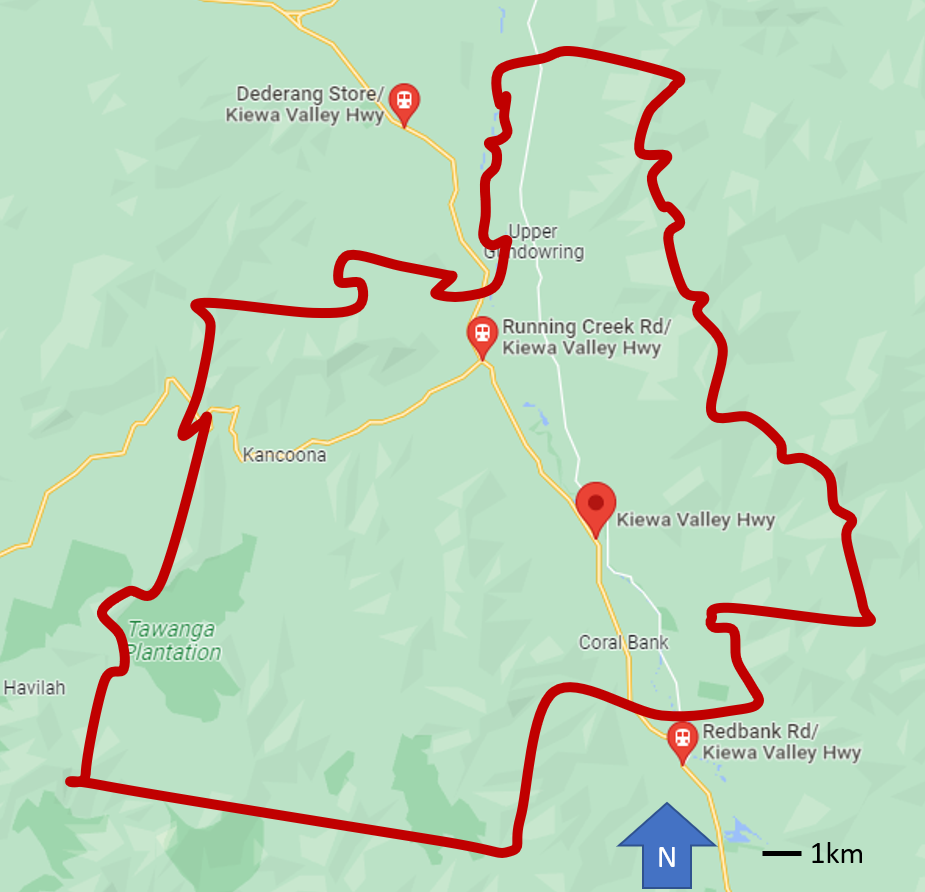
\includegraphics{images/Running_creek_bus_stop.png}
\caption{SA1 20403106915, with approximate location of Stop:ID 45125
highlighted, sources ABS and Google Maps}
\end{figure}

\begin{verbatim}
##   sa1_code_2021 sa2_code_2021         sa2_name_2021 sa3_code_2021
## 1   20403106915     204031069 Bright - Mount Beauty         20403
##      sa3_name_2021 sa4_code_2021 sa4_name_2021 gcc_code_2021 gcc_name_2021
## 1 Wodonga - Alpine           204          Hume         2RVIC  Rest of Vic.
##   state_code_2021 state_name_2021 areasqkm_2021  cent_lat cent_long
## 1               2        Victoria       284.598 -36.57879    147.05
\end{verbatim}

The area of SA1 20403106915 is 284.598km\textsuperscript{2}. By
inspection, the entire 400m radius catchment area of both of the bus
stops lie entirely within the SA1 20403106915 boundaries.

Hence the \(Area_{Bn}/ Area_{SA1_Area}\) term for each of the bus stops
is equal to \((\pi 400^2) / 284598000 =\) 1.77e-03.\\
No printed timetable has been located for the Albury - Mt Beauty via
Baranduda and Tawonga South route that services these stops, but stop
times are provided on the PTV website\^{}{[}See
\url{https://tinyurl.com/5n83ryhy}. This indicates services on Tuesday
August 8, 2023 to Albury at 7:25am, 9:25am and 9:30am and to Mt Beauty
at 2:50pm, 4:20pm and 4:40pm. In general, this appears to be a school
bus service pattern, with three services in each direction.Therefore the
total \(SI_{20403106915, 8/8/23}\) score is equal to
\((2*(6* pi * 400 * 400 / 284598000))\) which is equal to 0.0211943.

\hypertarget{exploring-the-results}{%
\subsection{Exploring the results}\label{exploring-the-results}}

To further review the quality of the output, the calculated scores were
briefly explored as follows:

\begin{itemize}
\item
  SI scores for SA1s within the Clayton (North) - Notting Hill
  Statistical Area Level 2 (SA2), in the vicinity of the Monash Clayton
  campus, were mapped and reviewed. This sub-unit of the case was
  selected as the area is familiar to members of the PTRG, and so could
  be relatively easily reviewed for any unexpected or anomalous results.
  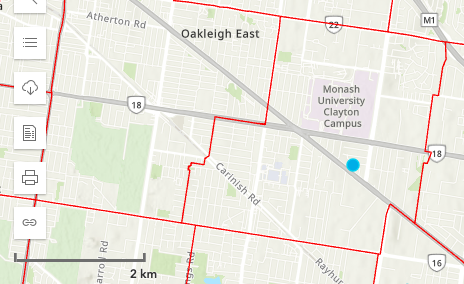
\includegraphics{images/Clayton.png}
\item
  Output results for SA1 zones within the Melbourne City Statistical
  Area Level 3 (SA3) were also examined. This SA3 includes Melbourne
  CBD, north Melbourne, Royal Park, Carlton, East Melbourne. parts of
  South Yarra and Prahan, and Southbank. Again, it has been selected for
  familiarity so as to help assess the accuracy of the reported SI
  results.
\end{itemize}

\begin{figure}
\centering
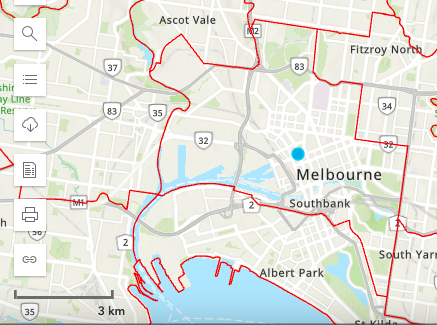
\includegraphics{images/Melbourne_city.png}
\caption{Melbourne City SA3 zone. Source: ABS.}
\end{figure}

\begin{itemize}
\tightlist
\item
  SI scores for SA1s within the Burwood (Vic.) SA2 area were also
  examined. This sub-unit of the case was selected as it contains the
  Burwood campus, and so the area is likely to be familiar to
  researchers from Deakin University. Hence it should provide a location
  where it is relatively easy for them to (also) review the SI scores
  for any unexpected or anomalous results.
\end{itemize}

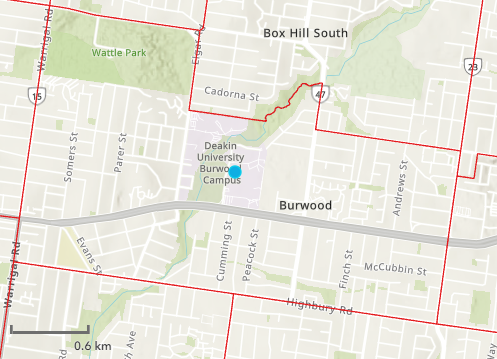
\includegraphics{images/Burwood.png} - SI scores for SA1s across all of
Greater Melbourne and all of Victoria were also explored. There are too
many SA1s to allow results to be clearly mapped, but some statistical
results are reported to, again, allow review for unexpected or anomalous
results.

\hypertarget{results}{%
\chapter{Results}\label{results}}

\hypertarget{verifing-the-code-output---running-creek}{%
\section{Verifing the code output - Running
Creek}\label{verifing-the-code-output---running-creek}}

The \(SI_{20403106915, 8/8/23}\) score calculated by the developed code
is shown in the following table.\\

\begin{table}

\caption{\label{tab:Running_Creek_SI_calc_SA1_2021}Developed code output for SA1 20403106915, August 8, 2023}
\centering
\begin{tabular}[t]{l|r|r|r|r|r|r|r|r|r|r|r}
\hline
sa1\_code\_2021 & LRT & subway & rail & bus & ferry & cable\_tram & aerial\_lift & funicular & trolleybus & monorail & Total\\
\hline
20403106915 & 0 & 0 & 0 & 0.0211944 & 0 & 0 & 0 & 0 & 0 & 0 & 0.0211944\\
\hline
\end{tabular}
\end{table}

The hand-calculated\footnote{See hand calculations in
  Methodology:Verifying the results section above.}
\(SI_{20403106915, 8/8/23}\) matches that produced by the developed
code, suggesting that the developed code is providing the expected
output. Checking the results for the same zone for 2018 to 2022
indicates an identical SI score for all but 2022, as shown in the
following tables.

\begin{table}

\caption{\label{tab:Running_Creek_SI_calc_SA1_2018_2022}Developed code output for SA1 20403106915, August 14, 2018}
\centering
\begin{tabular}[t]{l|r|r|r|r|r|r|r|r|r|r|r}
\hline
sa1\_code\_2021 & LRT & subway & rail & bus & ferry & cable\_tram & aerial\_lift & funicular & trolleybus & monorail & Total\\
\hline
20403106915 & 0 & 0 & 0 & 0.0211944 & 0 & 0 & 0 & 0 & 0 & 0 & 0.0211944\\
\hline
\end{tabular}
\end{table}

\begin{table}

\caption{\label{tab:Running_Creek_SI_calc_SA1_2018_2022}Developed code output for SA1 20403106915, August 13, 2019}
\centering
\begin{tabular}[t]{l|r|r|r|r|r|r|r|r|r|r|r}
\hline
sa1\_code\_2021 & LRT & subway & rail & bus & ferry & cable\_tram & aerial\_lift & funicular & trolleybus & monorail & Total\\
\hline
20403106915 & 0 & 0 & 0 & 0.0211944 & 0 & 0 & 0 & 0 & 0 & 0 & 0.0211944\\
\hline
\end{tabular}
\end{table}

\begin{table}

\caption{\label{tab:Running_Creek_SI_calc_SA1_2018_2022}Developed code output for SA1 20403106915, August 11, 2020}
\centering
\begin{tabular}[t]{l|r|r|r|r|r|r|r|r|r|r|r}
\hline
sa1\_code\_2021 & LRT & subway & rail & bus & ferry & cable\_tram & aerial\_lift & funicular & trolleybus & monorail & Total\\
\hline
20403106915 & 0 & 0 & 0 & 0.0211944 & 0 & 0 & 0 & 0 & 0 & 0 & 0.0211944\\
\hline
\end{tabular}
\end{table}

\begin{table}

\caption{\label{tab:Running_Creek_SI_calc_SA1_2018_2022}Developed code output for SA1 20403106915, August 10, 2021}
\centering
\begin{tabular}[t]{l|r|r|r|r|r|r|r|r|r|r|r}
\hline
sa1\_code\_2021 & LRT & subway & rail & bus & ferry & cable\_tram & aerial\_lift & funicular & trolleybus & monorail & Total\\
\hline
20403106915 & 0 & 0 & 0 & 0.0211944 & 0 & 0 & 0 & 0 & 0 & 0 & 0.0211944\\
\hline
\end{tabular}
\end{table}

\begin{table}

\caption{\label{tab:Running_Creek_SI_calc_SA1_2018_2022}Developed code output for SA1 20403106915, August 14, 2022}
\centering
\begin{tabular}[t]{l|r|r|r|r|r|r|r|r|r|r|r}
\hline
sa1\_code\_2021 & LRT & subway & rail & bus & ferry & cable\_tram & aerial\_lift & funicular & trolleybus & monorail & Total\\
\hline
20403106915 & 0 & 0 & 0 & 0.0211944 & 0 & 0 & 0 & 0 & 0 & 0 & 0.0211944\\
\hline
\end{tabular}
\end{table}

The SI scores for the Running Creek SA1 in each year match the hand
calculated score.

\hypertarget{clayton-north---notting-hill-sa2-supply-index-results-for-sa1s}{%
\section{Clayton (North) - Notting Hill SA2: Supply Index results for
SA1s}\label{clayton-north---notting-hill-sa2-supply-index-results-for-sa1s}}

This section briefly reviews the SI scores for SA1 zones within the
Clayton SA2 area. SI scores for the day of analysis in 2018 and 2023 are
compared in Figure \ref{fig:Clayton_SI_2021}.

\begin{figure*}
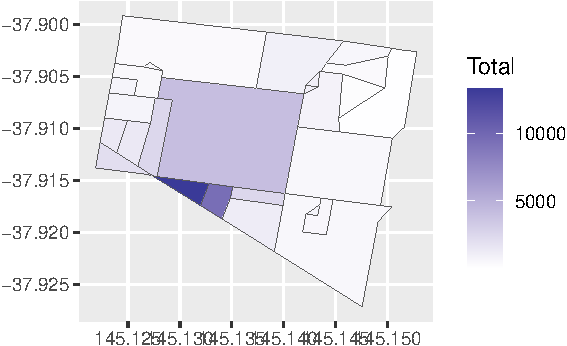
\includegraphics[width=0.5\linewidth]{Reynolds_Currie_2024_transit_supply_index_GTFS_files/figure-latex/Clayton_SI_2021-1} 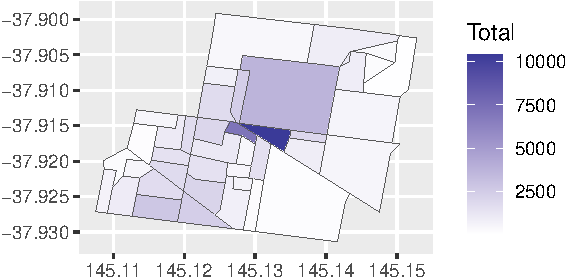
\includegraphics[width=0.5\linewidth]{Reynolds_Currie_2024_transit_supply_index_GTFS_files/figure-latex/Clayton_SI_2021-2} \caption[SI scores for SA1 zones within the Clayton SA2 area, 2018 (left) and 2023 (right)]{SI scores for SA1 zones within the Clayton SA2 area, 2018 (left) and 2023 (right)}\label{fig:Clayton_SI_2021}
\end{figure*}

The SI scores for SA1 zones within the Clayton SA2 area appear to meet
expectations. Higher scores are reported for SA1 zones that are close to
the Monash University bus loop (centre of the Clayton SA2 area) and near
the Clayton railway station (south-west of Clayton SA2 area). In general
there appear to have been little changes in SI between 2018 and 2023.

\begin{figure}
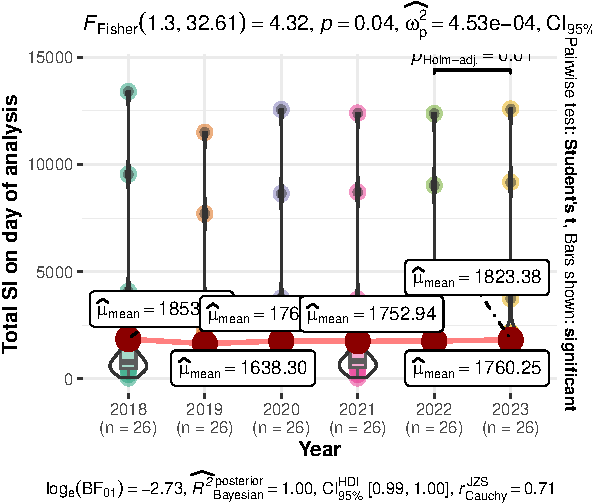
\includegraphics{Reynolds_Currie_2024_transit_supply_index_GTFS_files/figure-latex/Compare_2018_to_2023_Clayton_within_stats-1} \caption[SI scores for SA1 zones in the Clayton SA2 area, 2018 to 2023]{SI scores for SA1 zones in the Clayton SA2 area, 2018 to 2023: violin and box plot generated using ggstatsplot package}\label{fig:Compare_2018_to_2023_Clayton_within_stats}
\end{figure}

The box and violin plot (Figure
\ref{fig:Compare_2018_to_2023_Clayton_within_stats})indicates a
significant difference across the 2018 to 2023 scores for SA1s in the
Clayton North SA2 area. However, the differences appear to be small,
with scores in 2019, 2020, 2021 and 2022 generally lower than in 2018
and 2023. Perhaps this may relate to reductions in services during the
pandemic\footnote{The 601 Huntingdale to Clayton shuttle would appear
  likely to have had reduced service levels during lockdowns and prior
  to the resumption of on-campus teaching activity. However, this would
  not explain the low score in 2019, which predates the pandemic itself.
  Regardless, however, the changes appear to be generally small, so
  likely jus tto do with day-to-day operational variation.}.

\hypertarget{melbourne-city-sa3-supply-index-results-for-sa1s}{%
\section{Melbourne City SA3: Supply Index results for
SA1s}\label{melbourne-city-sa3-supply-index-results-for-sa1s}}

This section briefly reviews the SI scores for SA1 zones within the
Melbourne City SA3 area. SI scores for 2018 and 2023 are compared in
Figure \ref{fig:Melbourne_City_SI}.

\begin{figure*}
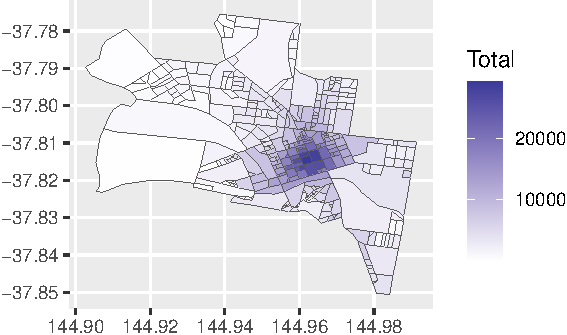
\includegraphics[width=0.5\linewidth]{Reynolds_Currie_2024_transit_supply_index_GTFS_files/figure-latex/Melbourne_City_SI-1} 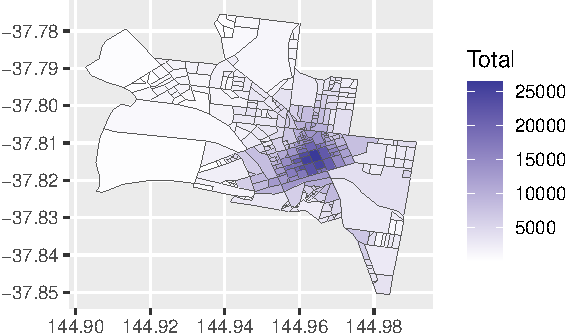
\includegraphics[width=0.5\linewidth]{Reynolds_Currie_2024_transit_supply_index_GTFS_files/figure-latex/Melbourne_City_SI-2} \caption[SI scores for SA1 zones within the Melbourne City SA3 area, 2018 (left) and 2023 (right)]{SI scores for SA1 zones within the Melbourne City SA3 area, 2018 (left) and 2023 (right)}\label{fig:Melbourne_City_SI}
\end{figure*}

The SI scores for SA1 zones within the Melbourne City SA3 area appear to
meet expectations. Higher scores are reported for SA1 zones in the
Melbourne CBD. In general there appear to have been little changes in SI
between 2018 and 2023.

\begin{verbatim}
## Error in integrate(marginal.g.oneWay, lower = 0, upper = Inf, F = F, N = N,  : 
##   non-finite function value
\end{verbatim}

\begin{figure}
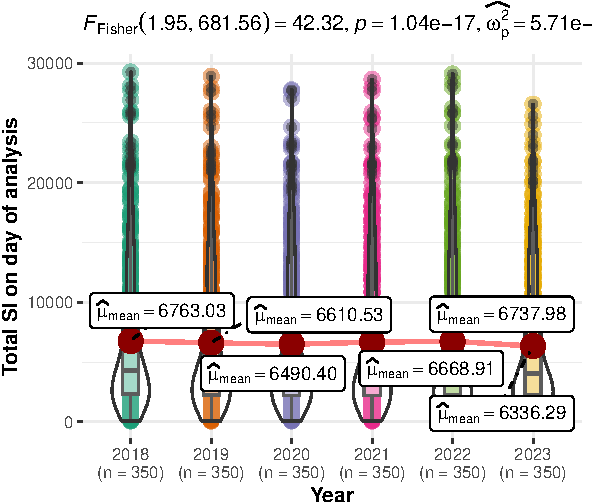
\includegraphics{Reynolds_Currie_2024_transit_supply_index_GTFS_files/figure-latex/Compare_2018_2023_Melbourne_City_within_stats-1} \caption[2018 through 2023 SI scores for SA1 zones in the Melbourne City SA3 area]{2018 through 2023 SI scores for SA1 zones in the Melbourne City SA3 area: violin and box plot generated using ggstatsplot package}\label{fig:Compare_2018_2023_Melbourne_City_within_stats}
\end{figure}

The box and violin plot (Figure
\ref{fig:Compare_2018_2023_Melbourne_City_within_stats}) indicates
significant differences across the 2018 through 2023 scores. However,
the differences appear to be small, and likely reflect minor changes to
services for operational reasons\footnote{The Melbourne Metro tunnel
  project has been ongoing through this time period, and has likely
  impacted on services along the Swanston Street tram corridor
  (especially with the works down at the Domain Interchange), around
  Flinders Street station and Melbourne Central Station.}.

\hypertarget{burwood-vic.-sa2-supply-index-results-for-sa1s}{%
\section{Burwood (Vic.) SA2: Supply Index results for
SA1s}\label{burwood-vic.-sa2-supply-index-results-for-sa1s}}

This section briefly reviews the SI scores for SA1 zones within the
Burwood (Vic.) SA2 area. SI scores for 2018 and 2023 are compared in
Figure \ref{fig:Burwood_SI}.

\begin{figure*}
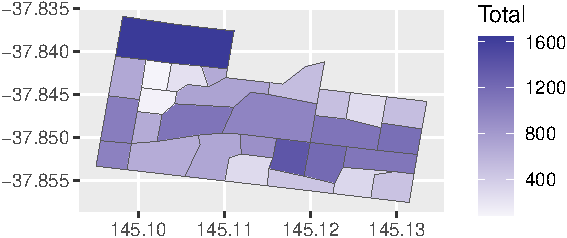
\includegraphics[width=0.5\linewidth]{Reynolds_Currie_2024_transit_supply_index_GTFS_files/figure-latex/Burwood_SI-1} 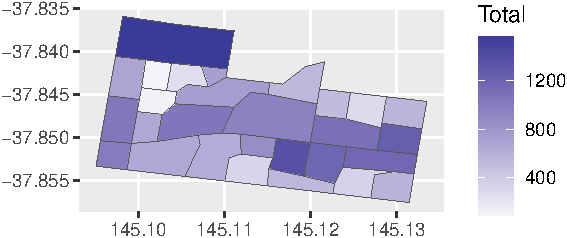
\includegraphics[width=0.5\linewidth]{Reynolds_Currie_2024_transit_supply_index_GTFS_files/figure-latex/Burwood_SI-2} \caption[SI scores for SA1 zones within the Burwood (Vic.) SA2 area, 2018 (left) and 2023 (right)]{SI scores for SA1 zones within the Burwood (Vic.) SA2 area, 2018 (left) and 2023 (right)}\label{fig:Burwood_SI}
\end{figure*}

The SI scores for SA1 zones within the Burwood (Vic.) SA2 area appear to
meet expectations. Higher scores are reported for SA1 zones along the
Burwood Highway corridor\footnote{The Burwood Highway runs east-west
  through centre of the maps.} and the SA1 zone to the
north-west\footnote{Tram route 70 runs along Riversdale Road to the
  north, which is likely the reason for the higher scores in the NW.} In
general there appear to have been little changes in SI between 2018 and
2023.

\begin{figure}
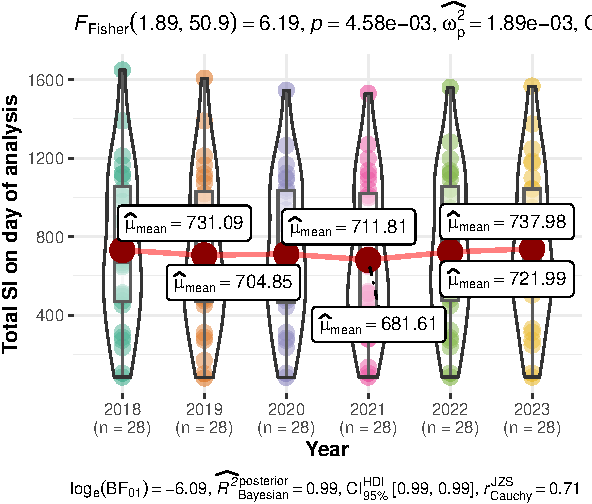
\includegraphics{Reynolds_Currie_2024_transit_supply_index_GTFS_files/figure-latex/Compare_2018_2023_Burwood_within_stats-1} \caption[2018 through 2023 SI scores for SA1 zones in the Melbourne City SA3 area]{2018 through 2023 SI scores for SA1 zones in the Melbourne City SA3 area: violin and box plot generated using ggstatsplot package}\label{fig:Compare_2018_2023_Burwood_within_stats}
\end{figure}

The box and violin plot (Figure
\ref{fig:Compare_2018_2023_Burwood_within_stats}) indicates significant
differences across the 2018 through 2023 scores. The mean scores are
lower in 2019 to 2021 than in 2018, 2022 and 2023. Some of this may be
related to minor service level alterations because of the COVID-19
pandemic, but in general the changes appear to be small and hence likley
to be associated with day-to-day operational variation across the years.

\hypertarget{greater-melbourne-and-all-of-victoria-supply-index-results-for-sa1s}{%
\section{Greater Melbourne and all of Victoria: Supply Index results for
SA1s}\label{greater-melbourne-and-all-of-victoria-supply-index-results-for-sa1s}}

Mapping SA1 scores across all of Victoria appears likely to result in
overwhelming detail, and so is not reported here. Hence, only the violin
and box plot is generated for all of Victoria.

\begin{verbatim}
## Error : vector memory exhausted (limit reached?)
## Error in h(simpleError(msg, call)) : 
##   error in evaluating the argument 'object' in selecting a method for function 'summary': vector memory exhausted (limit reached?)
\end{verbatim}

\begin{figure}
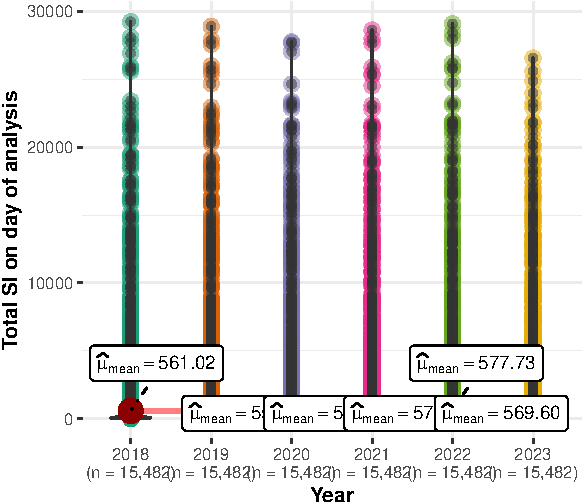
\includegraphics{Reynolds_Currie_2024_transit_supply_index_GTFS_files/figure-latex/Compare_2018_2023_Victoria_within_stats-1} \caption[2016 and 2021 SI scores for SA1 zones across Victoria]{2016 and 2021 SI scores for SA1 zones across Victoria: violin and box plot generated using ggstatsplot package}\label{fig:Compare_2018_2023_Victoria_within_stats}
\end{figure}

The box and violin plot (Figure
\ref{fig:Compare_2018_2023_Victoria_within_stats} indicates a
significant difference between the 2016 and 2021 scores for SA1 zones
across all of Victoria. The average score is higher in 2021 than it was
in 2016.

\hypertarget{discussion-and-conclusions}{%
\chapter{Discussion and Conclusions}\label{discussion-and-conclusions}}

This document presents preliminary results from the development of code
to calculate the \citet{currie2007identifying} transit Supply Index (SI)
directly from GTFS data. The developed code is available within the
Rmarkdown file used to typesset this document, and available on github.

The code out has been verified by performing hand calculations for SA1
SI scores in the Victorian Alps (Running Creek) and Talbot. The Running
Creek calculation, included two bus stops. This verification check
resulted in an exact match between the hand- and code-calculated values.

The verification calculation for Talbot involved regional train,
regional bus and local bus services across two bus stops and one train
station. The catchment areas for these stops and station were only
partially within the SA1. The hand-calculated and code-calculated SI
values were reasonably similar, with the different results likely due to
differing levels of precision in the assessment of areas and the lack of
available timetables for the service date in question. Further
verification checks, including more accurate assessment of catchment
area coverage, may be a direction for future research. Similarly,
additional verification calculations or close, step-by-step review of
the developed code may be a direction for future research.

The developed code was used to compare transit service levels for LGAs
across Greater Melbourne and the rest of Victoria at the time of 2016
and 2021 censuses. Results appear to be largely as might be expected,
with more transit service coverage generally being provided in more
central LGAs. There were significant differences between the 2016 and
2021 service levels across all of Victoria and for LGAs in Greater
Melbourne (average SI increased), but not for LGAs in Victoria but
outside Greater Melbourne.

Changes in SI scores appeared to be unevenly distributed across the
state, with outer regional areas having reduced service levels, while
some other LGAs, especially those in outer Melbourne, had higher SI
scores in 2021 than in 2016. There were significant changes in rail and
bus service levels between 2016 and 2021, but not for trams.

Some of the results suggest that the Overland train services (to
Adelaide) were not included in the GTFS file in 2021. It is unclear at
the moment whether this was because to the service was not operational,
or simply a data accuracy issue. However, this perhaps demonstrates the
challenge of using GTFS data alone for analysis of this nature: the
quality of the result is reliant on the quality of the underlying data.

Comparisons with IRSAD scores and ranks, and population suggest that SI
score is sificiantly associated with all three of these metrics. In
general, the SI increases with increases in population, IRSAD and IRSAD
rank, although it is important to note that increased IRSAD implies the
LGA has less social disadvantage. This would appear to be contrary to
what might be desired, with greater service provided to those areas
where there is greater disadvantage, but clearly there will be many
confounding factors and unclear causality involved in these
relationships. That said, Casey, Wyndham and Greater Geelong appear to
have particularly low SI scores given their residential population.

There is clearly much more anlaysis that can be done to expand on this
code. In particular, completing mapping of needs-gaps as per
\citet{currie2007identifying} would appear a promising direction for
future efforts. However, in general the verification calculations appear
to support the accuracy of the developed code, and the results from the
analysis suggest that output about Victorian LGAs is largely as might be
expected. Next steps appear to be to use GIS to improve the Talbot
verification calculations, and perhaps select a SA1 in Greater Melbourne
to do verification calculation on\footnote{This may be challenging
  though, as the hand-calculations are already quite involved, even for
  rural SA1s with only a few stops.}.

Additionally, the code will need to be forked so as to provide outputs
for Deakin\^{}\{2023 and 2018 SI scores for 7 days, using SA1 areas from
2021.\} and Monash\footnote{2021 and 2016 SI scores for 1 and 7 days,
  using SA1 areas from 2016.}. At approximately one day of processing
time per day of analysis, this would appear likely to take in the order
of 4-5 weeks\^{}\{Although I'm going to try to get a few different
computers going on this at the same time so that it takes less `real'
time.\}.

----\textgreater{}

\renewcommand\refname{References}
\bibliography{packages.bib,References.bib}



\end{document}
